% !TEX root = ../main.tex
\section{Q13: Regulering -- offentlig indgriben, branche-profit og political support}\label{q:13}

\begin{quote}
\emph{Præsentér økonomisk-teoretiske argumenter for hvornår offentlig indgriben i og regulering af markeder er hensigtsmæssig/anbefalelsesværdig samt for forudsætningerne bag disse argumenter. I forlængelse heraf ønskes en konkret præsentation af og redegørelse for modellen til beskrivelse af regulerede priser på baggrund af branche-profit-funktioner og political support-funktioner.}
\end{quote}

\subsection*{Svar (kort)}
Offentlig indgriben er hensigtsmæssig ved fire typer markedssvikt: naturlig monopol, eksternaliteter, offentlige goder og informasjonsasymmetri -- men kun under forutsætning av at reguleringsgevinsten overstiger reguleringsomkostningerne (government failure, regulatory capture). BSZ kap.\ 21-modellen viser at den regulerede prisen $P^*$ bestemmes der regulatoren (politikeren) maksimerer \emph{political support} $S(\pi, CS)$ -- en funksjon av brancheprofitt og konsumentoverskudd. Resultatet: $P^*$ ligger mellom $P^{MC}$ og $P^M$, avhengig av de relative lobbyingsressursene. [SLIDE]

\subsection*{Relevante teorier (kort)}

\paragraph{\thref{market-failure-regulation}{Markedssvikt og regulering}\quad\SOne}
Fire argumenter: (1) \textbf{Naturlig monopol}: fallende $AC$ $\Rightarrow$ én produsent billigst, men $P>MC$ uten konkurranse. Løsning: prisregulering, konsesjoner. (2) \textbf{Eksternaliteter} (\thref{externalities}{jf.\ Q07}): handlinger med uforprisede konsekvenser for tredjepart. Løsning: Pigou-skatt, kvoter. (3) \textbf{Offentlige goder}: ikke-rivaliserende, ikke-ekskluderbare $\Rightarrow$ free-riding. Løsning: offentlig tilbud. (4) \textbf{Informasjonsasymmetri} (\thref{adverse-selection}{adverse selection}): lemons, markedskollaps. Løsning: informasjonsplikt, sertifisering. Forutsetter at regulatoren er bedre informert og mer effektiv enn markedet -- noe som ikke alltid stemmer. [SLIDE/BOK]

\paragraph{\thref{regulated-pricing-model}{Regulated pricing-modellen (political support)}\quad\SOne}
BSZ kap.\ 21/Peltzman (1976): regulatoren maksimerer $S(\pi(P), CS(P))$. Brancheprofitt $\pi(P)$ er invers-U (null ved $P=AC$, topp ved $P^M$). Konsumentoverskudd $CS(P)$ er fallende. FOC: marginal politisk gevinst fra bransje ($\partial S/\partial \pi \cdot \pi'$) = marginal politisk kostnad fra konsumenter ($-\partial S/\partial CS \cdot CS'$). $P^*$ mellom $P^{MC}$ og $P^M$. Komparativ statikk: sterkere bransjelobby $\Rightarrow$ $P^*$ mot $P^M$; sterkere konsumentpress $\Rightarrow$ $P^*$ mot $P^{MC}$. [SLIDE/BOK]

\subsection*{Grafisk modell -- regulated pricing}

\begin{figure}[h]
\centering
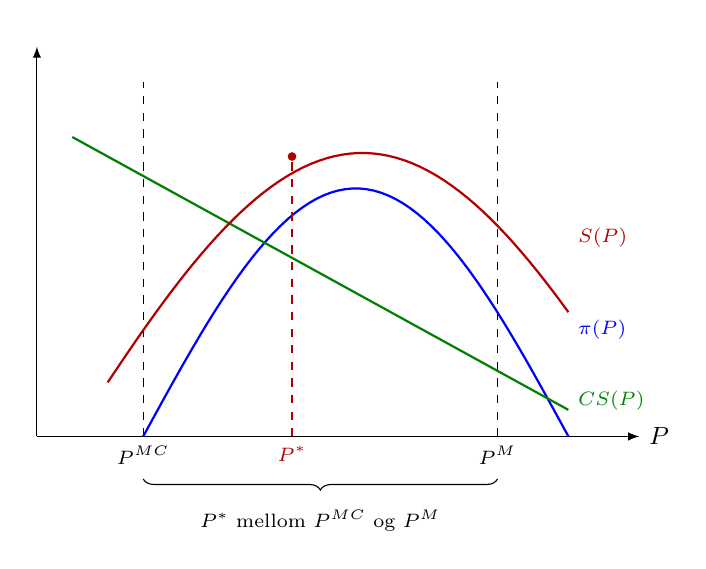
\begin{tikzpicture}[>=latex, scale=0.9, every node/.style={font=\small}]
  \draw[->] (0,0) -- (8.5,0) node[right] {$P$};
  \draw[->] (0,0) -- (0,5.5) node[above] {};
  % MC og PM
  \draw[dashed] (1.5,0) -- (1.5,5.0);
  \node[below] at (1.5,0) {\scriptsize $P^{MC}$};
  \draw[dashed] (6.5,0) -- (6.5,5.0);
  \node[below] at (6.5,0) {\scriptsize $P^{M}$};
  % pi(P)
  \draw[thick, blue, domain=1.5:7.5, samples=60]
    plot (\x, {3.5*sin((\x-1.5)*30)});
  \node[blue, right] at (7.5,1.5) {\scriptsize $\pi(P)$};
  % CS(P)
  \draw[thick, green!50!black, domain=0.5:7.5, samples=40]
    plot (\x, {4.5-0.55*\x});
  \node[green!50!black, right] at (7.5,0.5) {\scriptsize $CS(P)$};
  % S(P)
  \draw[thick, red!70!black, domain=1.0:7.5, samples=60]
    plot (\x, {4.0*sin((\x-0.5)*22)});
  \node[red!70!black, right] at (7.5,2.8) {\scriptsize $S(P)$};
  % P*
  \draw[thick, dashed, red!70!black] (3.6,0) -- (3.6,4.0);
  \node[below, red!70!black, font=\bfseries] at (3.6,0) {\scriptsize $P^{*}$};
  \filldraw[red!70!black] (3.6,3.95) circle (1.5pt);
  % Brace
  \draw[decorate, decoration={brace, amplitude=4pt, mirror}] (1.5,-0.6) -- (6.5,-0.6);
  \node[below, font=\scriptsize] at (4.0,-0.9) {$P^{*}$ mellom $P^{MC}$ og $P^{M}$};
\end{tikzpicture}
\caption{\textbf{Regulated pricing-modellen.} $\pi(P)$ (blå) topper ved monopolpris; $CS(P)$ (grønn) er fallende; $S(P)$ (rød) maksimeres ved $P^*$ mellom $P^{MC}$ og $P^M$. Regulatoren balanserer bransje- og konsumentinteresser. [BOK -- BSZ kap.\ 21]}
\end{figure}

\subsection*{De fire markedssviktene -- oversikt}

\begin{center}
\renewcommand{\arraystretch}{1.15}
\begin{tabular}{@{}p{3.0cm}p{3.5cm}p{3.0cm}p{3.5cm}@{}}
\toprule
\textbf{Svikt} & \textbf{Problem} & \textbf{Verktøy} & \textbf{Forutsætning} \\
\midrule
Naturlig monopol & $P>MC$, underprod. & Priskontroll & Fallende $AC$ \\
Eksternaliteter & Over-/underprod. & Pigou, kvoter & Tredjepartseffekt \\
Offentlige goder & Free-riding & Offentlig tilbud & Ikke-rival., ikke-ekskl. \\
Info.asymmetri & Lemons & Informasjonsplikt & Hidden info/action \\
\bottomrule
\end{tabular}
\end{center}

\subsection*{Real-world eksempler}

\textbf{Eks.~1 -- Norsk farmasiregulering.}\quad [EKS]
Statens legemiddelverk setter maksimale utsalgspriser (\emph{prisregulering}). Argumentet: naturlig monopol (patentbeskyttet legemiddel) + informasjonsasymmetri (pasienten kan ikke vurdere kvalitet). Prisen reflekterer political support-modellen: lavere enn USAs uregulerte priser (sterk konsumentinteresse, universell helseforsikring) men høyere enn generiske alternativ (bransjelobby for innovasjonsinsentiv). Forutsætningen er at regulatoren faktisk har bedre informasjon enn markedet -- kritikken er at industrien har informasjonsovertak og risikerer regulatory capture.

\textbf{Eks.~2 -- EU Emissions Trading System (ETS), sammenligning.}\quad [EKS]
ETS regulerer CO$_2$-utslipp (negativ eksternalitet) via kvotehandel -- en Pigou-mekanisme. Prisen ($\sim$50--80 EUR/tonn i 2024) er et politisk kompromiss mellom industriens profitt (høy kvotepris truer lønnsomhet) og konsumenter/klima (lav kvotepris gir for lite utslippsreduksjon). Sammenligningen med farmasiregulering: begge er political support-modellen i praksis, men med ulike markedssvikter (monopol vs.\ eksternalitet) og ulike verktøy (priskontroll vs.\ kvoter). I begge tilfeller avhenger $P^*$ av lobbyingsstyrke.

\subsection*{Kobling til Mærsk Power-to-X}
PtX mottar offentlige subsidier (EU Hydrogen Strategy, IPCEI) fordi grønt hydrogen produserer \emph{positive eksternaliteter} (klimareduksjon) som markedet underpriser. Reguleringsresponsen -- subsidie -- er korreksjonen for eksternaliteten. I tillegg er Mærsks PtX-satsing avhengig av at regulering av skipsdrivstoff (EU ETS Maritime, IMO) øker kostnaden ved fossil fuel (Pigou-skatt) og dermed gjør grønt alternativ kommersielt levedyktig. Political support-modellen forklarer hvorfor reguleringen er gradvis: skipsfartsbransjens lobby bremser innføringstakten, mens klimalobby presser den framover. [CASE]

\subsection*{Fallgruber}
\begin{itemize}\setlength{\itemsep}{2pt}
\item Glemme \emph{forudsætningerne} for at regulering er hensigtsmæssig -- sensor vil ha betingelsene, ikke bare argumentene.
\item Bare ramse opp de fire markedssviktene uten å forklare mekanismen (underproduksjon/overproduksjon/lemons).
\item Ignorere government failure, regulatory capture og Averch-Johnson -- regulering er ikke gratis.
\item Tegne modellen feil: $\pi(P)$ er \emph{invers-U}, ikke monotont stigende. $CS(P)$ er fallende, ikke stigende.
\item Glemme komparativ statikk: hva skjer med $P^*$ når lobbyingsstyrke endres?
\item Forveksle positiv analyse (``hva bestemmer regulert pris?'') med normativ (``hva bør regulert pris være?'') -- modellen er positiv (Peltzman), ikke normativ (Pigou).
\end{itemize}

\subsection*{Håndskrivbar disposisjon (15-min forberedelse)}
\begin{itemize}\setlength{\itemsep}{2pt}
\item \textbf{Tese:} Regulering hensigtsmæssig ved 4 markedssvikter, men betinget av at reguleringsgevinst > reguleringsomkostning. Modellen viser at $P^*$ er politisk kompromiss, ikke velferdsmaksimum.
\item \textbf{4 svikter:} (1) Naturlig monopol ($AC$ fallende). (2) Eksternaliteter (Pigou). (3) Offentlige goder (free-rider). (4) Info.asymmetri (lemons).
\item \textbf{Forutsætninger:} signifikant svikt, regulatoren informert, ikke capture.
\item \textbf{Modell:} $\pi(P)$ invers-U; $CS(P)$ fallende; $S(\pi, CS)$ maksimeres ved $P^*$. FOC: $\partial S/\partial\pi \cdot \pi' = -\partial S/\partial CS \cdot CS'$.
\item \textbf{Komparativ statikk:} sterkere lobby $\Rightarrow$ $P^*\to P^M$; sterkere konsument $\Rightarrow$ $P^*\to P^{MC}$.
\item \textbf{Kritikk:} government failure, capture (Stigler), AJ-overinvestering, Olsons kollektiv handling.
\item Eks.\ 1: Norsk farmasiregulering (monopol + info.asym.). Eks.\ 2: EU ETS (eksternalitet).
\item Case: Mærsk PtX -- subsidier for pos.\ eksternalitet + IMO-regulering som Pigou.
\item Søyle: \SOne\ (regulatoren allokerer rettigheter stat/marked).
\end{itemize}
